% !TEX encoding = UTF-8
% !TEX TS-program = pdflatex
% !TEX root = ../tesi.tex

\subsection{UC3 - Visualizzazione file}
\begin{itemize}
  \item \textbf{Identificativo}: UC3
  \item \textbf{Nome}: visualizzazione file
  \item \textbf{Descrizione grafica}:
\end{itemize}

\begin{figure}[h]
  \centering
  %  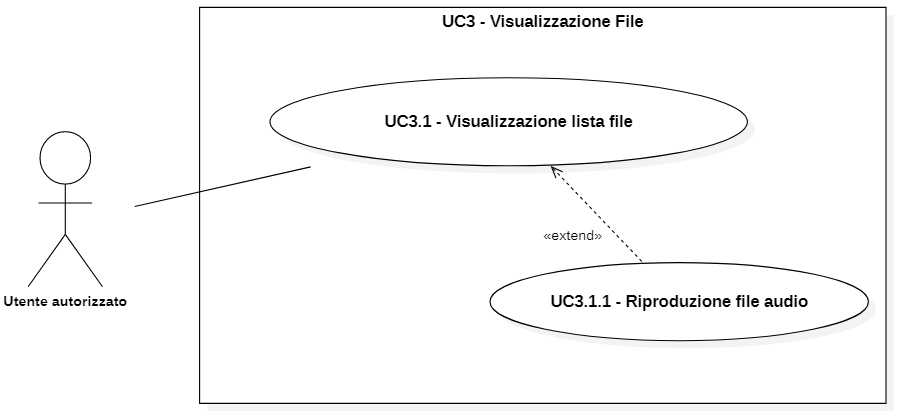
\includegraphics[scale=0.50]{images/UC3.png}
  \caption{Descrizione grafica caso d'uso UC3}
\end{figure}

\begin{itemize}
  \item \textbf{Attori}
        \begin{itemize}
          \item \textit{Primari}: utente autorizzato
        \end{itemize}
  \item \textbf{Precondizione}: l'utente si trova sulla pagina per il caricamento dati, che ha già effettuato correttamente.
  \item \textbf{Postcondizione}: l'utente visualizza i file e i relativi metadati caricati.
  \item \textbf{Scenario principale}: l'utente ha caricato correttamente i dati, questi vengono visualizzati con una lista di file ognuno con i relativi metadati.
  \item \textbf{Scenario secondario}: l'utente può visualizzare ed elaborare i metadati relativi ad ogni file \textbf{UC5}.
\end{itemize}

\subsubsection{UC3.1 - Visualizzazione lista file}
\begin{itemize}
  \item \textbf{Identificativo}: UC3.1
  \item \textbf{Nome}: visualizzazione lista file
  \item \textbf{Descrizione grafica}: (approfondita in UC3)
  \item \textbf{Attori}
        \begin{itemize}
          \item \textit{Primari}: utente autorizzato
        \end{itemize}
  \item \textbf{Precondizione}: l'utente si trova sulla pagina per il caricamento dati, che ha già effettuato correttamente.
  \item \textbf{Postcondizione}: l'utente visualizza la lista dei file ognuno con i relativi metadati.
  \item \textbf{Scenario principale}: l'utente visualizza la lista dei file e può visualizzare la lista dei metadati associati.
  \item \textbf{Scenario secondario}: l'utente può riprodurre i file audio \textbf{UC3.1.1}.
\end{itemize}

\subsubsection{UC3.1.1 - Riproduzione audio file}
\begin{itemize}
  \item \textbf{Identificativo}: UC3.1.1
  \item \textbf{Nome}: riproduzione audio file
  \item \textbf{Descrizione grafica}: (approfondita in UC3)
  \item \textbf{Attori}
        \begin{itemize}
          \item \textit{Primari}: utente autorizzato
        \end{itemize}
  \item \textbf{Precondizione}: l'utente si trova sulla pagina per il caricamento dati, che ha già effettuato correttamente.
  \item \textbf{Postcondizione}: il file audio viene riprodotto.
  \item \textbf{Scenario principale}: l'utente comanda il riproduttore audio con gli appositi comandi play/pause.
\end{itemize}

[Manca visualizzazione/modifica codici procedimenti da capire come gestire questo caso d'uso]